\chapter{Barèmes}
\label{annexe:baremes}

\section{Barème pour la sécurité}
\label{annexe:baremes_securite}

L'équation suivante donne une équation exponentielle où la droite passe nécessairement par ($a$,0) et ($c$,1). Le ratio $a/b$ peut être ajusté pour donner la forme voulue à la courbe.
\begin{equation}
    y(x) = \frac{e^{\frac{x-a}{b}-1}}{e^{\frac{c-a}{b}-1}}
    \label{annexe:bareme_sécurité}
\end{equation}

Dans le cas où $c=5$,

\begin{figure}[h]
    \centering
    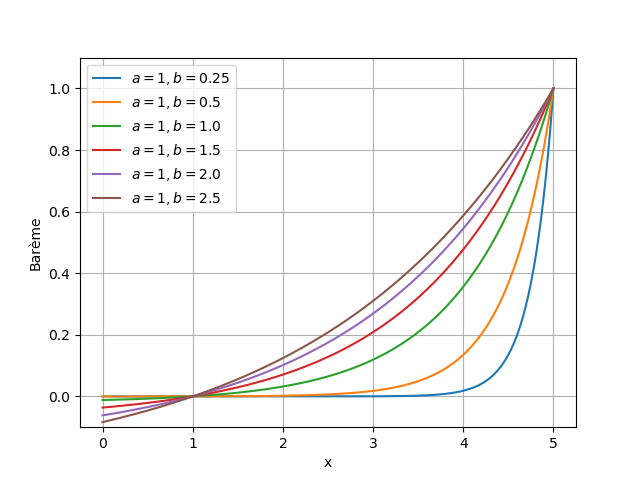
\includegraphics[width=0.75\linewidth]{fig/exp_securite.png}
    \caption{Barème exponentielle pour la sécurité}
    \label{fig:exp_securite}
\end{figure}

\section{Barème pour la taille des poissons}
\label{annexe:baremes_poisson}


L'équation suivante donne une équation exponentielle où la droite passe nécessairement par (0,1) et ($a$,0). Le ratio $a/b$ peut être ajusté pour donner la forme voulue à la courbe.
\begin{equation}
    y(x) = \frac{1-10^{\frac{x-a}{b}}}{1-10^{a/b}}
    \label{annexe:bareme_exp_poisson}
\end{equation}

\begin{figure}[h]
    \centering
    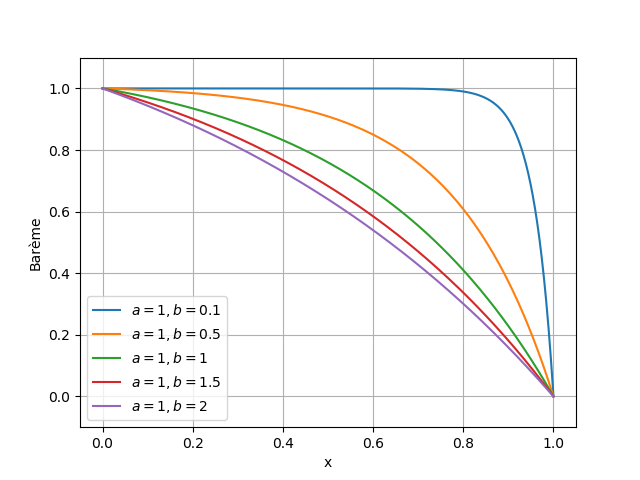
\includegraphics[width=0.75\linewidth]{fig/exp_poisson.png}
    \caption{Barème exponentielle pour la taille des poissons}
    \label{fig:exp_poisson}
\end{figure}

